%!TEX root=../GaugeCNNTheory.tex

\subsubsection*{هموردایی سراسری دورانی و مقیاسی روی $\Euc_2 \backslash \{0\}$ از طریق مختصات لگاریتمی-قطبی}
\label{sec:polar_Euc2_logpolar}

\begin{figure}
	\centering
	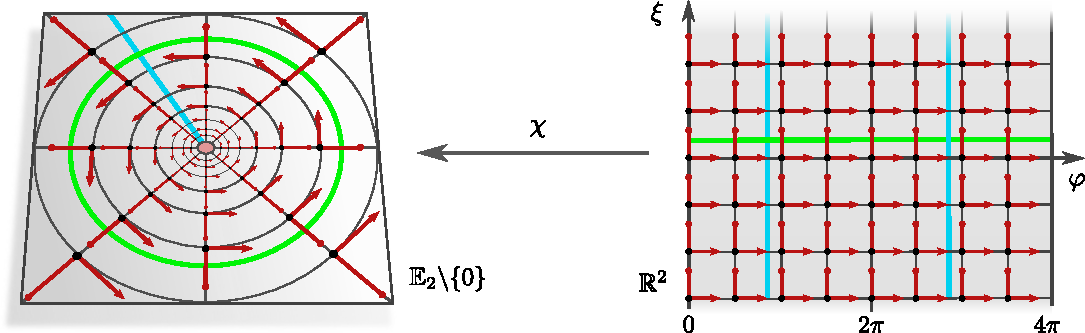
\includegraphics[width=.94\textwidth]{figures/G_structure_R2_no_origin_logpolar_coords.pdf}
	\vspace*{2ex}
	\caption{\small
		مختصات لگاریتمی-قطبی 
		$\chi: \R^2 \to \R^2 \backslash \{0\} :\, (\varphi,\xi) \mapsto \big( e^{\xi}\cos(\varphi) ,\, e^{\xi}\sin(\varphi) \big)$
		زوایای $\varphi \in \R$ و لگاریتم-شعاع‌های $\xi = \log\lVert p\rVert \in \R$ را به نقاط $p$ در $\R^2 \backslash \{0\}$ نگاشت می‌دهد.
		پس از انتخاب مختصات دکارتی برای $\Euc_2 \backslash \{0\} \cong \R^2 \backslash \{0\}$، این کار یک مختصاتی‌سازی از $\Euc_2 \backslash \{0\}$ توسط $\R^2$ به دست می‌دهد.
		مختصات لگاریتمی-قطبی یک $\{e\}$-ساختار را روی $\Euc_2 \backslash \{0\}$ القا می‌کند که شامل چارچوب‌های مرجع
		$\big[ \frac{\partial}{\partial \varphi} ,\, \frac{\partial}{\partial \xi} \big]$ است که با شبکه مختصاتی تراز شده‌اند.
		آنها علاوه بر این یک متریک ریمانی را القا می‌کنند که با متریک اقلیدسی معمول متفاوت است و چارچوب‌های القا شده نسبت به آن راست‌هنجار هستند.
		کانولوشن‌های $\GM$ روی این $\{e\}$-ساختار متناظر با کانولوشن‌های اقلیدسی متعارف در مختصات $\R^2$ هستند.
		انتقال‌های $(\Delta\varphi,\, \Delta\xi) \in \Trans_2$ در $\R^2$ از طریق $\chi$ متناظر با دوران‌ها و تغییرمقیاس‌های $\Euc_2 \backslash \{0\}$ هستند، که در آن زوایای دوران و فاکتورهای تغییرمقیاس به ترتیب با $\Delta\varphi$ و $e^{\Delta\xi}$ داده می‌شوند.
		بنابراین، هموردایی انتقالی کانولوشن در مختصات $\R^2$ بر هموردایی ${\SO2 \!\times\! \Scale}$ کانولوشن $\GM$ روی $\Euc_2 \backslash \{0\}$ دلالت دارد.
		این نتیجه با هموردایی ایزومتری کانولوشن $\GM$ مطابقت دارد زیرا تبدیلات در $\IsomGM = {\SO2 \!\times\! \Scale}$ نسبت به متریک القا شده، ایزومتری هستند.
		\citet{esteves2017polar} چنین کانولوشن‌های $\GM$ را بر حسب کانولوشن‌های متعارف روی $\R^2$ پیاده‌سازی می‌کنند.
	}
	\label{fig:G_structure_R2_no_origin_logpolar}
\end{figure}

با ناوردا کردن $G$-ساختارهای ناوردای دورانی از بخش قبل نسبت به مقیاس، کانولوشن‌های $\GM$ متناظر نسبت به گروه حاصلضرب مستقیم ${\SO2 \!\times\! \Scale}$ هموردا می‌شوند.
چنین $G$-ساختارهایی توسط \emph{مختصات لگاریتمی-قطبی} القا می‌شوند، که در شکل~\ref{fig:G_structure_R2_no_origin_logpolar} نشان داده شده است و امکان یک پیاده‌سازی راحت از کانولوشن $\GM$ را بر حسب کانولوشن‌های اقلیدسی متعارف روی نمایش مختصاتی $\R^2$ فراهم می‌کند.
هموردایی انتقالی کانولوشن‌ها روی $\R^2$ سپس متناظر با هموردایی ${\SO2 \!\times\! \Scale}$ روی $\Euc_2 \backslash \{0\}$ است.
برای وضوح، ما با توصیف مدل بر حسب مختصات لگاریتمی-قطبی همانطور که توسط \citet{esteves2017polar} پیشنهاد شده، شروع می‌کنیم.%
\footnote{
	ایده پیاده‌سازی همبستگی‌های ناوردای دورانی از طریق تبدیلات لگاریتمی-قطبی پیش از این در دهه ۸۰ میلادی ظاهر شده بود~\cite{saito1983scale,casasent1987real}.
}
متعاقباً، ما بررسی می‌کنیم که چگونه این مدل و ویژگی‌های آن در چارچوب ما توضیح داده می‌شوند.

مختصات لگاریتمی-قطبی فضای برداری اقلیدسی سوراخ‌دار $\R^2 \backslash \{0\}$ بر حسب پوشای هموار زیر تعریف می‌شود:
\begin{align}
	\chi:\, \R^2 \to \R^2 \backslash \{0\} \,,\ \ 
	(\varphi, \xi) \mapsto \big( e^\xi \cos(\varphi) ,\, e^\xi \sin(\varphi) \big) \,,
\end{align}
که نقاط $p = \chi(\varphi,\xi)$ را در $\R^2 \backslash \{0\}$ به یک زاویه قطبی داده شده $\varphi \in \R$ و لگاریتم-شعاع ${\xi = \log\lVert p\rVert \in \R}$ اختصاص می‌دهد.
این نگاشت در مختصات زاویه‌ای $2\pi$-متناوب است (به تکرار نوار آبی در سمت راست شکل~\ref{fig:G_structure_R2_no_origin_logpolar} توجه کنید) و بنابراین به طور خاص یک‌به‌یک نیست.
یک تحدید به $[0,2\pi) \times \R$ دوسویه و پیوسته خواهد بود، اما همسان‌ریخت نخواهد بود -- این امر ما را ملزم می‌کند که در ادامه حداقل دو چارت را برای پوشش صفحه سوراخ‌دار در نظر بگیریم.
مختصات دکارتی $\R^2 \backslash \{0\}$ را با $\Euc_2 \backslash \{0\}$ یکی می‌گیرد و بنابراین اجازه می‌دهد که مختصات لگاریتمی-قطبی به دومی اختصاص داده شود.
از آنجا که سیستم‌های مختصات دکارتی مختلف (راست‌گرد) که در مبدأ $\Euc_2 \backslash \{0\}$ متمرکز شده‌اند فقط در دوران‌ها متفاوت هستند، تخصیص مختصات لگاریتمی-قطبی با یک جابجایی در مؤلفه زاویه‌ای مبهم است.

با توجه به یک نقشه ویژگی $f: \R^2 \backslash \{0\} \to \R^c$ (یک میدان ویژگی مرتبط با $\eM$، همانطور که در ادامه روشن می‌شود)، \citet{esteves2017polar} پول‌بک آن $\tilde{f} := f \circ \chi \ : \R^2 \to \R^c$ را از طریق مختصات لگاریتمی-قطبی در نظر می‌گیرند، که توسط جابجایی نمودار زیر تعریف می‌شود:
\begin{equation}
	\begin{tikzcd}[row sep=2.5em, column sep=5.em]
		\R^2
		\arrow[r, "\chi"]
		\arrow[rr, bend left=20, "\tilde{f}"', pos=0.3]
		& \R^2 \backslash \{0\}
		\arrow[r, "f"]
		& \R^c
	\end{tikzcd}
\end{equation}
یک کانولوشن گروهی هموردای دورانی و مقیاسی از میدان ویژگی~$f$ روی $\R^2 \backslash \{0\}$ سپس به صورت زیر تعریف می‌شود:
۱) پول‌بک آن از طریق $\chi$ به مختصات $\R^2$
۲) اعمال یک کانولوشن اقلیدسی متعارف در آنجا و
۳) نگاشت نتیجه به $\R^2 \backslash \{0\}$.
این روش خوش‌تعریف است زیرا $\chi$ هموار است، به طوری که نقشه‌های ویژگی (میدان‌های ویژگی) هموار $f$ منجر به پول‌بک‌های هموار و متناوب $\tilde{f}$ می‌شوند.
از آنجا که کانولوشن‌ها مستقل از موقعیت هستند، نقشه ویژگی خروجی آنها همچنان متناوب و هموار خواهد بود و بنابراین به طور یکتا به یک نقشه ویژگی هموار روی $\R^2 \backslash \{0\}$ متناظر است.%
\footnote{
	برای دیدن این موضوع، توجه داشته باشید که $\chi$ یک نگاشت خارج‌قسمتی است (زیرا بخش زاویه‌ای آن یک نگاشت خارج‌قسمتی $\R \to S^1 \cong \R/2\pi\mathbb{Z}$ است).
	برای نقشه‌های ویژگی پیوسته (به جای هموار) این گزاره از ویژگی جهانی فضاهای خارج‌قسمتی نتیجه می‌شود؛ به عنوان مثال به 
	\href{https://en.wikipedia.org/wiki/Quotient_space_(topology)\#Properties}{\underline{ویکی‌پدیا}}
	مراجعه کنید.
	از آنجا که همواری یک تابع به عنوان مشتق‌پذیری پیوسته آن تعریف می‌شود، ویژگی جهانی را می‌توان به صورت بازگشتی اعمال کرد تا نشان دهد که این گزاره برای نقشه‌های ویژگی هموار نیز برقرار است.
}

هموردایی دورانی و مقیاسی کانولوشن گروهی ضمنی روی $\R^2 \backslash \{0\}$ از هموردایی انتقالی تابع مختصاتی~$\chi$ نتیجه می‌شود.%
\footnote{
	اینکه این امکان‌پذیر است به این واقعیت بستگی دارد که یک همومورفیسم گروهی
	$\Trans_2 \to \SO2 \!\times\! \Scale,\ (\Delta\varphi,\, \Delta\xi) \mapsto (R_{\Delta\varphi},\, e^{\Delta\xi})$
	وجود دارد که توسط ایزومورفیسم گروهی $\exp: \Trans_1 \to \Scale$ روی عامل دوم و همومورفیسم گروهی (نگاشت خارج‌قسمتی) $R: \Trans_1 \to \SO2 \cong \Trans_1 / 2\pi\mathbb{Z}$ روی عامل اول تعریف می‌شود، که در آن $R_{\Delta\varphi}$
	ماتریس دوران با زاویه $\Delta\varphi$ را نشان می‌دهد.
}
فرض کنید $(\varphi, \xi)$ هر مختصاتی در $\R^2$ باشد و $(\Delta\varphi, \Delta\xi)$ هر انتقالی در $\Trans_2$ باشد.
نقطه $\R^2 \backslash \{0\}$ که متناظر با مختصات منتقل شده ${(\varphi \!+\! \Delta\varphi} ,\, {\xi \!+\! \Delta\xi)}$ است، سپس به نقطه متناظر با مختصات منتقل نشده $(\varphi, \xi)$ از طریق یک مقیاس‌بندی با ضریب $e^{\Delta\xi}$ و دوران با زاویه $\Delta\varphi$ مرتبط می‌شود:
\begin{align}\label{eq:log_polar_translation_equivariance}
	\chi \big( \varphi+\Delta\varphi ,\, \xi+\Delta\xi \big)
	&= e^{\xi+\Delta\xi} \begin{pmatrix} \cos(\varphi+\Delta\varphi) \\ \sin(\varphi+\Delta\varphi) \end{pmatrix} \notag \\
	&= e^{\Delta\xi}
	\begin{pmatrix} \cos(\Delta\varphi)\mkern-8mu & -\sin(\Delta\varphi) \\ \sin(\Delta\varphi)\mkern-8mu & \phantom{-} \cos(\Delta\varphi) \end{pmatrix}
	e^\xi \begin{pmatrix} \cos(\varphi) \\ \sin(\varphi) \end{pmatrix} \notag \\
	&= e^{\Delta\xi}
	\begin{pmatrix} \cos(\Delta\varphi)\mkern-8mu & -\sin(\Delta\varphi) \\ \sin(\Delta\varphi)\mkern-8mu & \phantom{-} \cos(\Delta\varphi) \end{pmatrix}
	\chi(\varphi,\, \xi) \notag \\
	&=: (\Delta\varphi,\, \Delta\xi) \,\rhd\, \chi(\varphi,\, \xi)
\end{align}
بر حسب یک نمودار، این بدان معناست که
\begin{equation}
	\begin{tikzcd}[row sep=3.5em, column sep=7.em]
		\R^2
		\arrow[r, "{(\Delta\varphi {,}\, \Delta\xi) +}"]
		\arrow[d, "\chi"']
		& \R^2
		\arrow[d, "\chi"]
		\\
		\R^2 \backslash \{0\}
		\arrow[r, "{(\Delta\varphi {,}\, \Delta\xi) \rhd}"']
		& \R^2 \backslash \{0\}
	\end{tikzcd}
\end{equation}
برای انتقالات دلخواه، جابجایی است.
این به همراه هموردایی انتقالی کانولوشن‌های متعارف روی $\R^2$ دلالت بر این دارد که نقشه‌های ویژگی ورودی دوران یافته و مقیاس شده روی $\R^2 \backslash \{0\}$ منجر به نقشه‌های ویژگی خروجی دوران یافته و مقیاس شده روی $\R^2 \backslash \{0\}$ خواهند شد، یعنی هموردایی ${\SO2 \!\times\! \Scale}$ کانولوشن روی $\R^2 \backslash \{0\}$.
جزئیات بیشتر در مورد این دیدگاه در~\cite{esteves2017polar} و~\cite{blatt1994canonical} یافت می‌شود.

اکنون این عملیات کانولوشن و ویژگی‌های آن را از دیدگاه کانولوشن‌های $\GM$ مستقل از مختصات بازبینی می‌کنیم.
برای این کار، یک اطلس از چارت‌ها را در نظر می‌گیریم که با مختصات لگاریتمی-قطبی سازگار هستند و $\{e\}$-ساختار، پیمانه‌ها، متریک ریمانی، ژئودزیک‌ها و انتقال موازی القا شده توسط آن را مورد بحث قرار می‌دهیم.
هموردایی ادعا شده ${\SO2 \!\times\! \Scale}$ بلافاصله از هموردایی $\IsomeM$ کانولوشن‌های $\GM$ نتیجه می‌شود.
برای راحتی نمادگذاری، ما دوباره $\Euc_2 \backslash \{0\}$ را از طریق یک انتخاب از مختصات دکارتی با $\R^2 \backslash \{0\}$ یکی می‌گیریم.

از آنجا که تحدید $\tilde{\chi}: [0,2\pi) \times \R \to \R^2 \backslash \{0\}$ از مختصات لگاریتمی-قطبی $\chi$ به زوایای غیرزائد، دوسویه و پیوسته است، ممکن است وسوسه شویم که وارون آن را به عنوان یک چارت مختصاتی در نظر بگیریم.
این کار، با این حال، ممکن نیست، زیرا $\tilde{\chi}$ یک همسان‌ریختی نیست، همانطور که برای چارت‌ها لازم است.
در عوض، ما یک اطلس متشکل از دو چارت را در نظر می‌گیریم که بر حسب تحدیدهایی از $\chi$ تعریف شده‌اند و $\R^2 \backslash \{0\}$ را پوشش می‌دهند.
یک انتخاب خاص، تعریف هم‌دامنه‌های چارت به عنوان مجموعه‌های باز $V^A = (0,2\pi) \times \R$ و $V^B = (-\epsilon,\epsilon) \times \R$ برای یک $0< \epsilon <\pi$ است و برای $X=A,B$ تعریف چارت‌ها روی $U^X = \chi(V^X)$ به صورت $x^X := \big( \chi\big|_{V^X} \big)^{-1} : U^X \to V^X$ است.
به طور شهودی، این اطلس همان کاری را انجام می‌دهد که تلاش ساده‌لوحانه برای تعریف چارت‌ها به عنوان وارون $\tilde{\chi}$ انجام می‌داد.
تفاوت مهم، با این حال، این است که چارت‌ها دیفئومورفیک هستند، که برای اطمینان از همواری تمام عملیات ضروری است.

طبق معمول، این چارت‌ها میدان‌های چارچوب محلی و تریویالیزاسیون‌های کلاف را به ترتیب روی $U^A$ و $U^B$ القا می‌کنند.
به راحتی می‌توان دید که نگاشت‌های گذار $g_p^{BA} = \frac{\partial x^B}{\partial x^A} |_{x^A(p)}$ روی $U^A \cap U^B$ بدیهی هستند، که این نتیجه می‌دهد که اجتماع میدان‌های چارچوب یک $\{e\}$-ساختار هموار $\eM$ را روی $\R^2 \backslash \{0\}$ تعریف می‌کند.
این پایه‌های مختصاتی، که در مقالات اغلب با $\big[ \frac{\partial}{\partial \varphi} ,\, \frac{\partial}{\partial \xi} \big]$ نشان داده می‌شوند، در شکل~\ref{fig:G_structure_R2_no_origin_logpolar} (چپ) نشان داده شده‌اند.
محاسبه ما در معادله~\eqref{eq:log_polar_translation_equivariance} در بالا دلالت بر این دارد که $\{e\}$-ساختار القا شده ${\SO2 \!\times\! \Scale}$-ناوردا است.

چارت‌ها علاوه بر این یک متریک ریمانی را القا می‌کنند که با متریک اقلیدسی معمول روی $\R^2 \backslash \{0\}$ متفاوت است.
این متریک به عنوان پول‌بک متریک اقلیدسی $\langle \cdot,\cdot \rangle_{\R^2}$ در هم‌دامنه‌های چارت‌ها تعریف می‌شود و بنابراین به صورت نقطه‌ای با
\begin{align}
	\eta_p(v,w) \,:=\, \big\langle \hat{d}x^X_p(v) \,,\, \hat{d}x^X_p(w) \big\rangle_{\R^2} \,,
\end{align}
داده می‌شود، که در آن $v,w \in \TpM$ و $X$ هر یک از چارت‌هایی را که $p\in U^X$ نشان می‌دهد، مشخص می‌کند.
$\{e\}$-ساختار القا شده توسط چارت، بنا به ساختار، از \emph{چارچوب‌هایی تشکیل شده است که نسبت به این متریک القا شده توسط چارت، راست‌هنجار هستند}، حتی اگر این \emph{چارچوب‌ها با افزایش شعاع هنگام اندازه‌گیری نسبت به متریک اقلیدسی استاندارد، رشد کنند}.
اتصال لوی-چیویتا برای متریک القا شده با اتصال اقلیدسی معمول متفاوت است و بنابراین ژئودزیک‌ها و انتقال‌دهنده‌های موازی جایگزینی را نتیجه می‌دهد.
از آنجا که متریک از طریق چارت‌ها پول‌بک می‌شود، ژئودزیک‌ها متناظر با خطوط مستقیم در هم‌دامنه‌های چارت‌ها هستند -- یک مثال، خطوط مختصاتی روی $\R^2 \backslash \{0\}$ در شکل~\ref{fig:G_structure_R2_no_origin_logpolar} است.
انتقال موازی نیز متناظر با انتقال معمول در هم‌دامنه‌های چارت‌ها است، که این نتیجه می‌دهد که بردارهای منتقل شده را در یک زاویه ثابت نسبت به خطوط مختصاتی روی $\R^2 \backslash \{0\}$ نگه می‌دارد؛ پاورقی~\ref{footnote:punctured_Euclidean_transport} را مقایسه کنید.
توجه داشته باشید که این همان انتقالی است که قبلاً در مدل‌های متناظر با شکل‌های~\ref{fig:G_structures_R2_no_origin} در بالا مورد بحث قرار گرفت، که در آنجا انتقال متناظر با اتصال لوی-چیویتا \emph{نبود} زیرا آن مدل‌ها متریک استاندارد را روی $\R^2 \backslash \{0\}$ به جای متریک القا شده توسط چارت فرض می‌کردند.

ایزومتری‌های حافظ $\{e\}$-ساختار $\IsomeM \cong {\SO2 \!\times\! \Scale}$ \emph{نسبت به متریک القا شده توسط چارت} با دوران‌ها و تغییرمقیاس‌های $\{e\}$-ساختار \emph{نسبت به متریک اقلیدسی معمول} داده می‌شوند.
قضیه~\ref{thm:isom_equiv_GM_conv} بر هموردایی ${\SO2 \!\times\! \Scale}$ کانولوشن $\GM$ متناظر دلالت دارد -- که گزاره بیان شده توسط \citet{esteves2017polar} را در نظریه ما بازیابی می‌کند.
همانطور که در بالا گفته شد، این واقعیت که متریک از طریق چارت‌ها القا می‌شود به این معنی است که تمام عملیات هنگام بیان در چارت به عملیات اقلیدسی معمول خلاصه می‌شوند.
بنابراین کانولوشن $\GM$ به بهترین وجه از طریق یک کانولوشن متعارف روی چارت پیاده‌سازی می‌شود، همانطور که توسط \citet{esteves2017polar} پیشنهاد شده است.

توجه داشته باشید که هموردایی ${\SO2 \!\times\! \Scale}$ کانولوشن $\GM$ به راحتی به هموردایی ${\O2 \!\times\! \Scale}$ که شامل بازتاب‌ها نیز می‌شود، قابل تعمیم است.
این کار با انجام یک کانولوشن هموردای بازتابی در چارت پیاده‌سازی می‌شود، که متناظر با $\Flip$-ساختار نشان داده شده در شکل~\ref{fig:G_structure_R2_3} است.
روی $\R^2 \backslash \{0\}$، این امر به یک $\Flip$-ساختار منجر می‌شود که شبیه به ساختار در شکل~\ref{fig:G_structure_R2_no_origin_O2} در بالا است، با این تفاوت که $\Flip$-ساختار علاوه بر این تحت یک تغییرمقیاس سراسری نیز ناوردا است.